%!TEX root = ../master.tex
\chapter{Implementation}\label{ch:implementation}
Our development chapter. \todo{We describe Rear Infused Illumination, and add all theory we have on the things mention if RID - for example BLOBs, contrast, illumination and so on.}

\section{Rear Diffused Illumination} \label{sec:RDI}
The interaction on the game board table will be based on rear diffused illumination as described in Multi-Touch Technologies \citep{multiTT}. As shown in figure ((ref project sketch)) this means we are going to make inputs in the augmented board game via having it recognise the touch of the board as BLOBs shown in IR light. This is because of a camera beneath the table's surface that observes a change in the contrast shown in IR light. 
For this to work, the table's top surface, made of transparent material, needs a diffuser material just above or beneath it in order to diffuse the light. Infra-red light then needs to be shone on it from beneath the surface. When the glass is pressed from above the surface by an object, that part of the surface reflects more light back which will be captured by the camera as a BLOB.
\begin{figure}[!h]
\centering	\includegraphics[width=0.5\textwidth]{sketchAugmentedBoard}
\label{Fig:sketch} \caption{An sketch of our RDI table.}
\end{figure}

Choosing such a solution has it's advantages and disadvantages. First of all, there is no need for a compliant surface or soldering for a LED frame, since we are using a diffuser in order to reflect the IR-light coming from below. The illuminators for that can be bought ready to go, so there is no need to build them. A disadvantage comes from the RDI having difficulties with getting even illumination, since the IR-lights might cover the table's surface completely. This can result in false BLOBs and BLOBs of lower contrast, which will challenge the software's detection of the real BLOBs.

\section{Physical Design} 
\begin{figure} [!h]
\centering 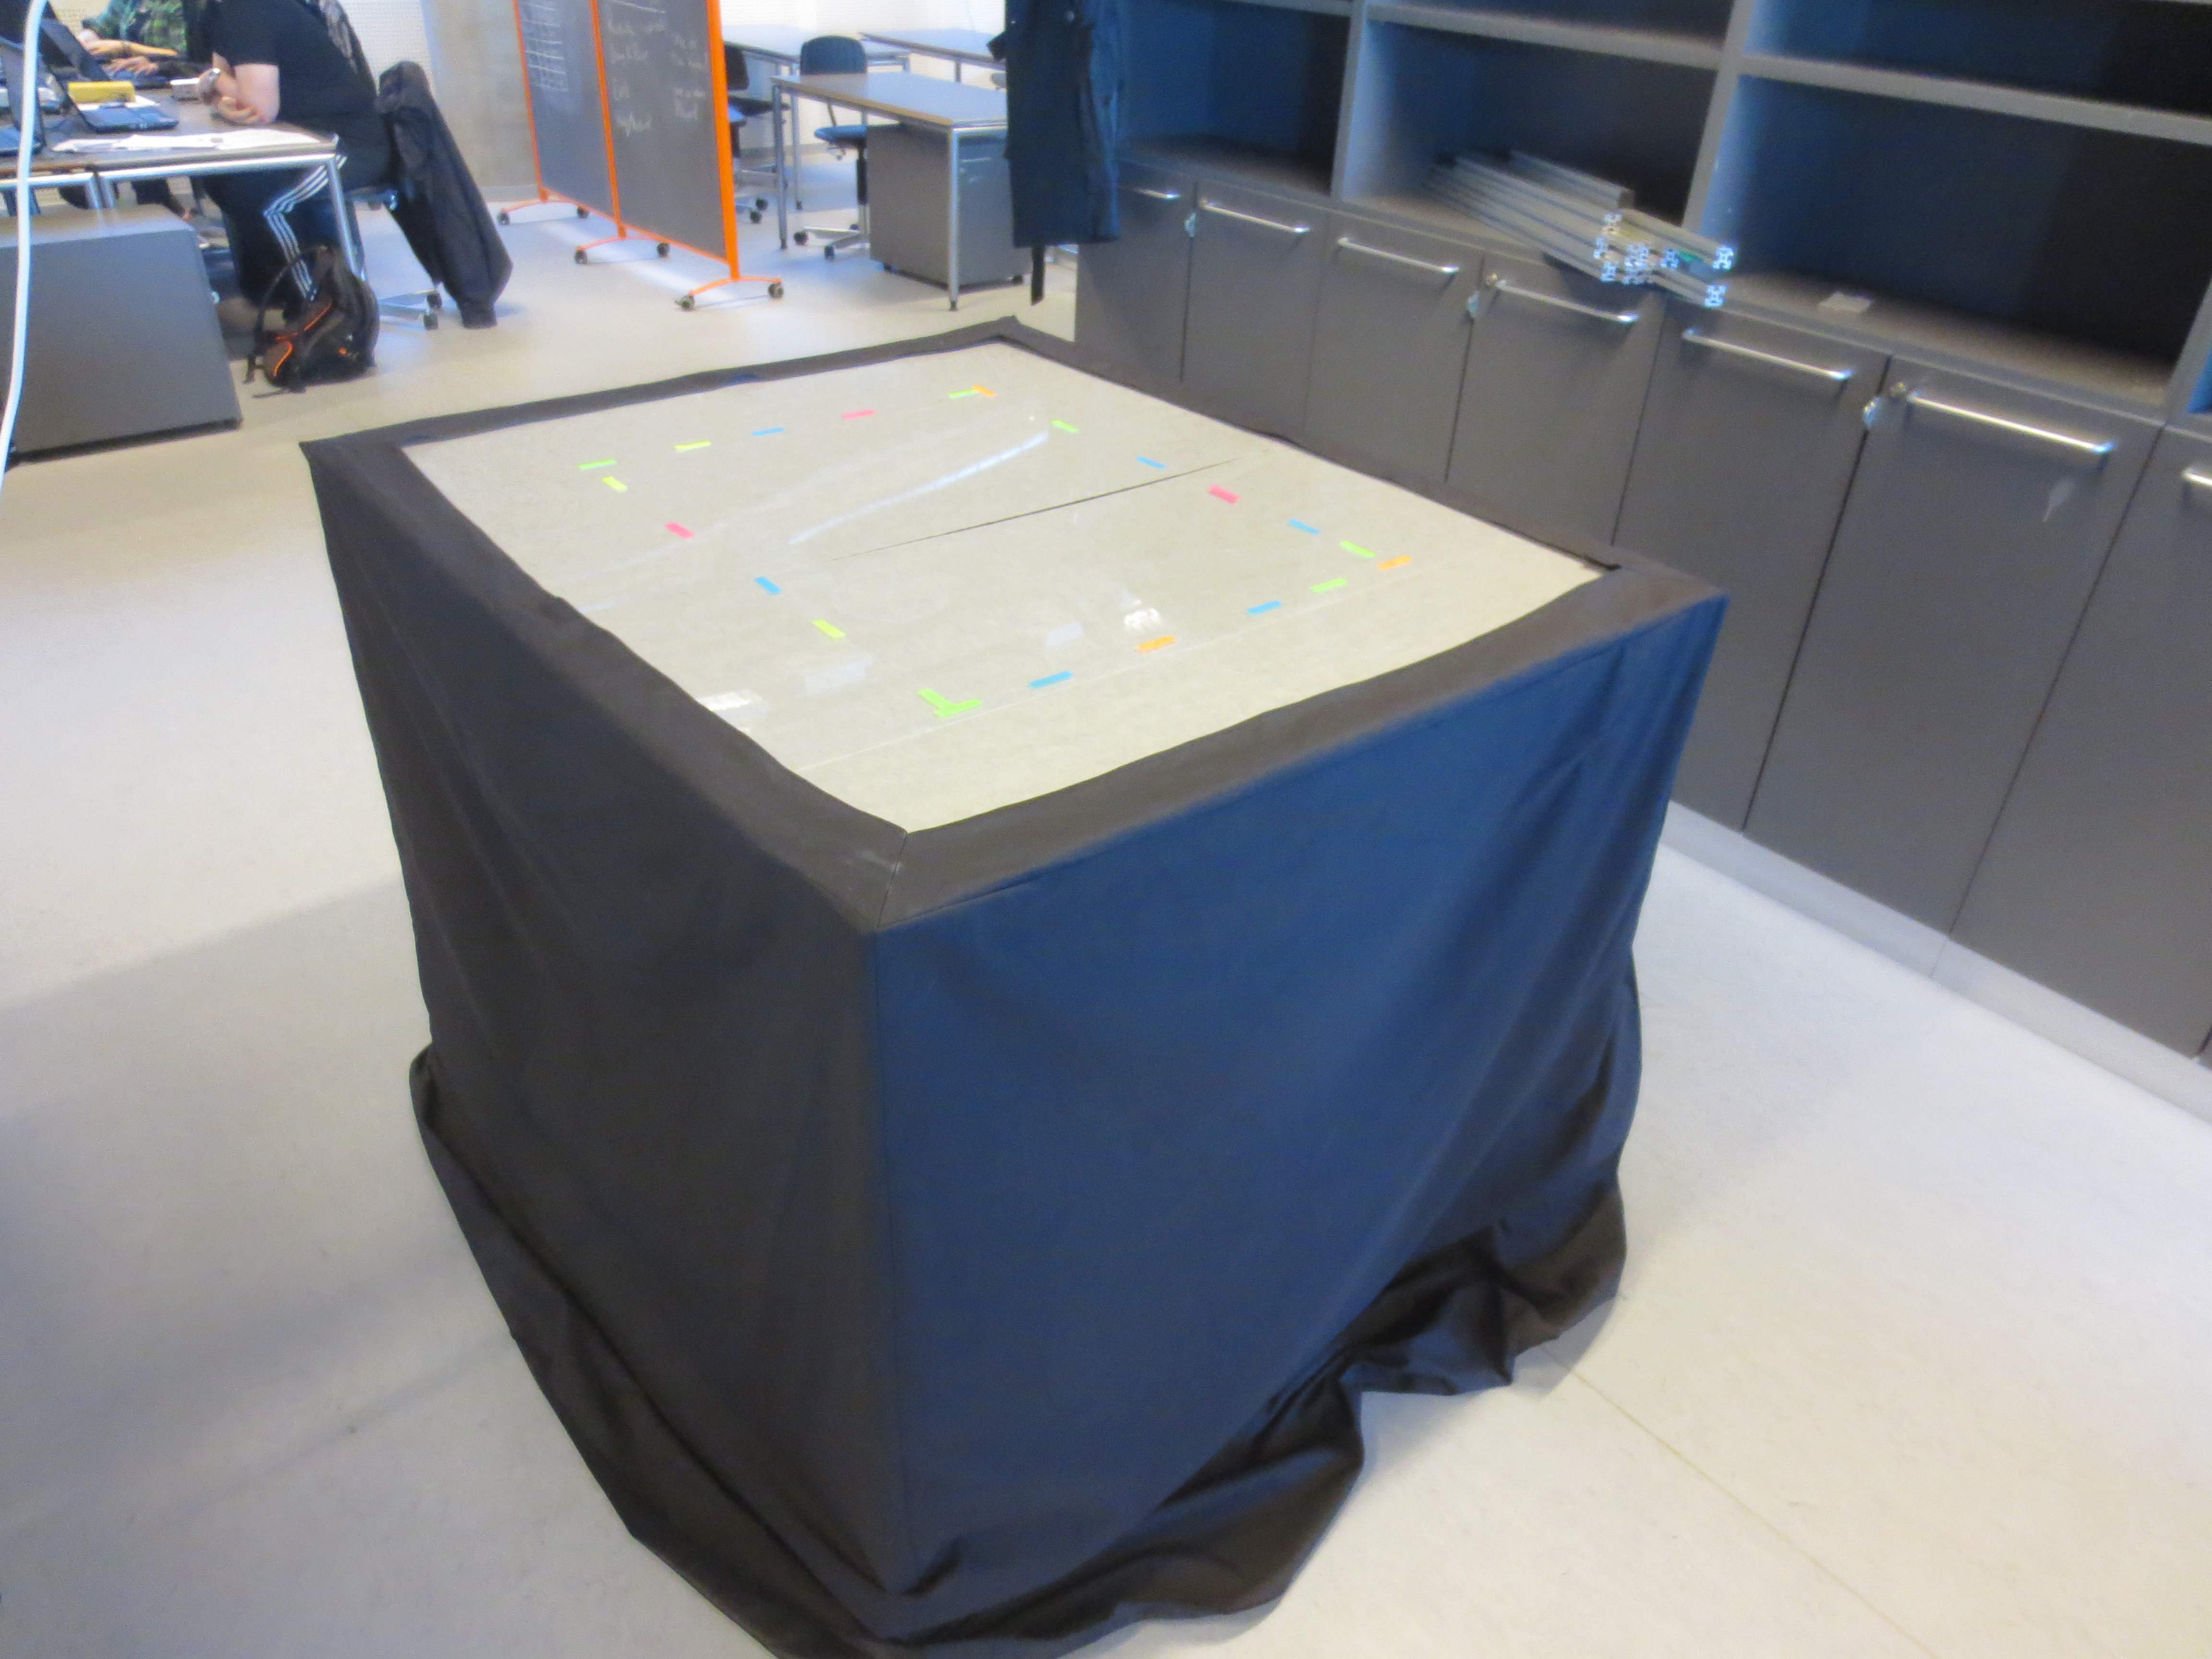
\includegraphics[width=0.5\textwidth]{Table}
\label{Fig:Table} \caption{The touch table}
\end{figure}
This section will describe the physical aspect of our product.
We have assembled a touch board, made with a acrylic glass top and IR lamps below. Underneath the surface of the top is a short-throw projector so we are able to project images on the table. Additionally we have a webcam with an IR filter placed at the very bottom of the table, so we are able to detect, what is happening on the table surface. This is thanks to the reflected IR light, as explained in section \ref{sec:RDI}.

The outer frame of the table is constructed from 3 different lengths of aluminium rods, giving the table a final size of 120 x 102 x 89 cm.
After the outer frame of the table was assembled, a cloth cover was made for the table. The cover was made to make the inside af the table darker, so a better projection was achieved and to prevent the IR light from damaging peoples eyes. To be able to test the interior, diffusing material was needed on the acrylic glass top. Baking paper was chosen for this job\todo{please describe why.}. The baking paper was attached on the bottom of the acrylic glass top, meaning that the user wouldn't be able to feel the baking paper when they interact with the board. 
With the exterior finished, it was time for the interior to be constructed. The positions of the electronics were decided and the interior was build, based on what gave the best results. 

During the construction of the table, a few problems were encountered. One of the problem encountered was that the baking paper did not sit tight against the acrylic glass and was slowly falling down. This gave us problems when trying to reflecting IR light from it. The problem was fixed by taping the baking paper to the acrylic glass with duct tape. 

\section{Image Processing}
To facilitate user interaction, a software module is needed to analyse a video input and recognize specific features and changes in it over time. There are two main criteria for this software. It needs to:
\begin{itemize}
\item Recognize specific finger touches.
\item Recognize specific game pieces.
\end{itemize}

To do this, BLOBs need to be extracted from the video input through segmentation. Since it is difficult to create a uniform surface of reflected IR-light, it might be necessary to apply a filter to the input before segmentation. Furthermore, since this is a video feed rather than a static image, changes in illumination may need to be accounted for as well. This leads to a four-step solution for processing the video input:
\begin{enumerate}
\item Prepare video frame for segmentation (Pre-segmentation).
\item Segment image (Segmentation).
\item Remove noise from the segmented image (Post-segmentation).
\item Analyse BLOB(s) (BLOB-analysis).
\end{enumerate}

\subsection{Segmentation methods}
There are several methods for segmenting images. Relevant methods are discussed in this section. Since this project deals with video as opposed to static images, a single threshold with a fixed threshold value is not useful. The hardware setup uses Rear Diffused Illumination with infrared light sources, and an  infrared filter on a web camera. This should create an ideal image for segmentation using an automatic global thresholding method. This method makes use of the histogram of an image to identify the most optimal threshold value\citep{Moeslund2012c4}. In an ideal image, the histogram will have two distinct 'mountains' of pixel values, that is to say, there will be two groups of pixels that, within each group, have a similar brightness while at the same time the groups themselves are isolated from each other. In the case of this project, the image produced should have bright spots where the board is touched, on a dark plane which is to be considered the background. The software then needs to identify an optimal threshold value between these two groups. One such method, is to evaluate the Figure~\ref{eq:otsu} for each brightness value in the histogram. The result with the lowest value is then selected.
\begin{figure}[h]
	\begin{align}
	C(T)&=M_1(T)\cdot\sigma_1^2(T)+M_2(T)\cdot\sigma_2^2(T)
	\end{align}
	\caption{$M_1(T)$ is is the number of pixels left of $T$ and $M_2(T)$ is the number of pixels to the right. $\sigma_1^2(T)$ and $\sigma_2^2(T)$ is the variance of the pixels to the left and right repsectively \label{eq:otsu} \citep[p. 61]{moeslund_introduction_2012_chapter_5}}
\end{figure}

